\section{Introduction}

\label{Section: introduction}
%With the increasing demand for continuous video analytics in public safety and transportation, more and more cameras are being deployed to various locations. The video analytics are based on classical computer vision techniques as well as deep convolutional neural networks. In recent years, we have also witnessed the emergence of a large number of excellent models for target detection \cite{trade-offs}, such as FasterRCNN \cite{ren2015faster_rcnn}, RFCN \cite{dai2016r_fcn}, Multibox \cite{szegedy2014multibox}, SSD \cite{liu2016ssd} and YOLO \cite{redmon2016yolo}.
%For the collected video, the classical computer vision and deep neural network technology are generally used for video analytics. 
A video analytics application consists of a \emph{pipeline} of several video processing modules, typically including a decoder, a selective sampling frame application, and a target detector. Such a pipeline always has multiple \emph{knobs}, such as frame rate, resolution,  detector model selection and so on. A combination of the knob values is video analytics \emph{configuration}, and the configuration space grows \emph{exponentially} with the number of knobs and their values \cite{jiang2018chameleon}.
%(e.g., SSD \cite{liu2016ssd}+{MobileNet \cite{MobileNetV2}, ResNet \cite{he2016resnet}\}, FasterRCNN \cite{ren2015faster_rcnn}+\{ResNet \cite{he2016resnet},InceptionResNet \cite{szegedy2016inception}\}).

Different configurations directly affect accuracy and resource consumption. The best configuration is the one with the lowest resource demand whose accuracy is over the desired threshold, whcih can optimize the \emph{trade-off} between accuracy and energy consumption. The \emph{best} configuration for video analysis services often varies in minutes or even seconds \cite{jiang2018chameleon}. As shown in Figure~\ref{fig: framework}(a), if one uses an expensive static configuration (e.g., only profiles the processing pipeline \emph{once} to choose the high frame rate and image resolution) can be precise, but it can also be a huge drain on resource consumption. Similarly, specifying a cheap static configuration (e.g., low resolution and small model) will significantly reduce accuracy. The framework of our solution %To tackle these challenges, we propose an adaptive configuration approach, AdaConfigure, and the brief framework
is shown in Figure~\ref{fig: framework}(b), and we tackle the following design challenges.

\begin{figure*}[!t]
	%\begin{tabular}{cc}
	\begin{minipage}{\linewidth}
		\centerline{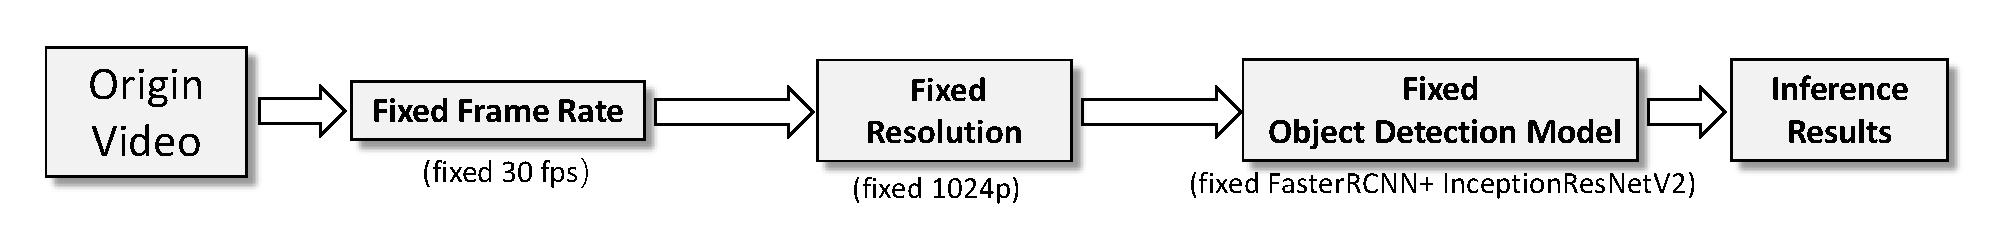
\includegraphics[width=0.9\linewidth]{figures/static_framework.pdf}}
		\begin{center}
			{(a) Static configuration solution: fixed configuration for video analytics services}
		\end{center}
		%        \vspace{0.3cm}
	\end{minipage}
	\vfill
	\vspace{0.4cm}
	\begin{minipage}{\linewidth}
		\centerline{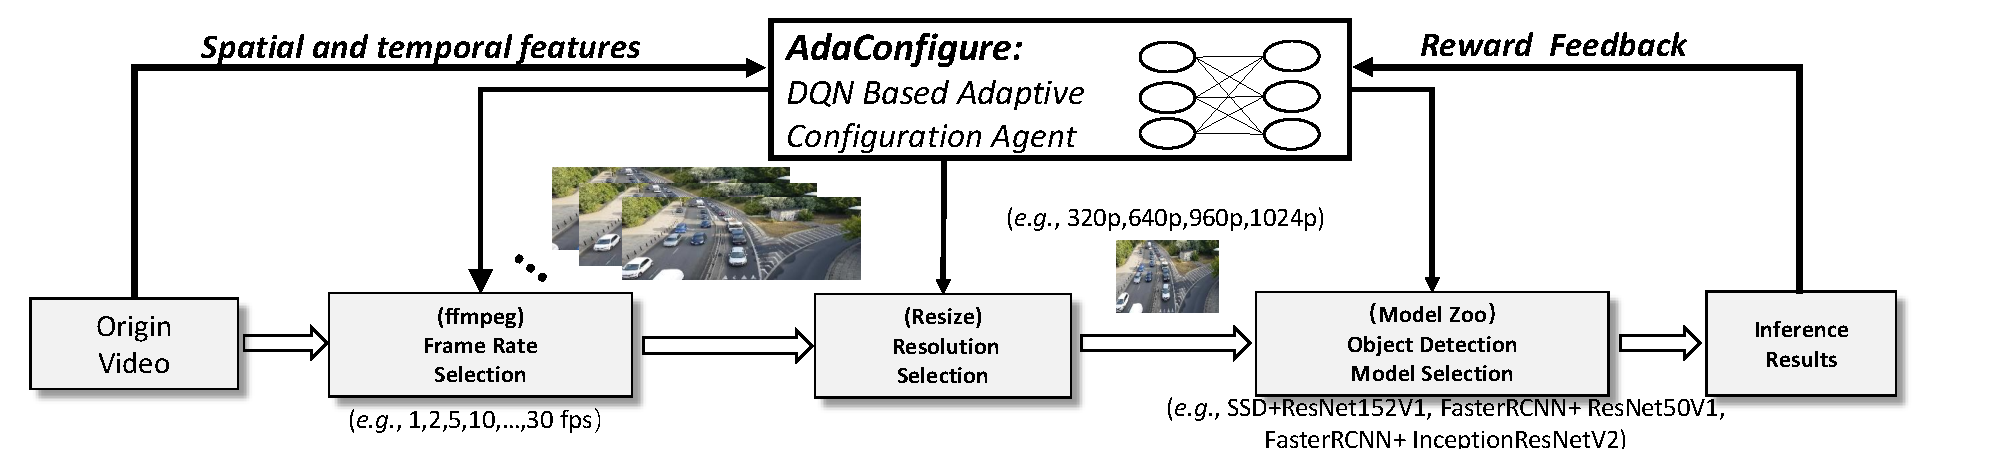
\includegraphics[width=0.9\linewidth]{figures/auto_framework.pdf}}
		\vspace{0.2cm}
		\begin{center}
			{(b) AdaConfigure solution: reinforcement learning-based adaptive configuration framework}
		\end{center}
	\end{minipage}
	%\end{tabular}
	%\vspace{0.1cm}
	\caption{Comparing to the static solution, our solution can adaptively update the configuration strategy based on the reward feedback}
	%	\caption{Comparing to the static solution, our solution can update the configuration strategy based on the object detection model feedback}
	\label{fig: framework}
	\vspace{-0.5cm}
\end{figure*}

\emph{Choosing the best configuration is a complicated decision-making problem that is challenging to be solved by rules.} The best configuration for video analytics services changes significantly because the exact context of the videos varies over time and across space. For instance, tracking vehicles when traffic moves quickly requires a higher frame rate than when traffic moves slowly. Spatially, the characteristics of video content are different in different locations. For instance, cameras in downtown areas show more cars than the other cameras deployed in the suburbs. It is hard to make an exact rule to choose a configuration for the current context by profiling such complicated video characteristics.
%	but each condition may vary by hour, minute, even second.
%As a dynamic video analytics configuration %solution
%application, we target to provide a solution that dynamically picks a configuration according to intrusive dynamics of video context, i.e., it can \emph{generate} video analytics configuration for video analytics in a different time.

\emph{Adaptive configuration would cause a huge extra overhead.} The number of possible configurations grows exponentially, and thousands of configurations can be combined with just a few knobs \cite{jiang2018chameleon}. So exhaustive periodically (e.g., profile once per 4 seconds) configuration to find the best configuration is a highly unrealistic approach because it causes a huge extra overhead, which may exceed the benefits of adaptive configurations. To significantly reduce the resource cost for adaptive configuration requires one solution that automatically chooses a configuration instead of manually trying using various configurations, which is challenging to previous studies including \cite{jiang2018chameleon,wang2020jcab}, since their approaches pay attention to reduce search space algorithm, and try various configurations in search space to find the best configuration.
%using a brute-force search (i.e., periodically trying various configurations and selecting the one with the best performance)

%\setlist{nolistsep}
%\begin{itemize}	
%	\item \emph{Choosing the best configuration is a complicated decision-making problem that is challenging to be solved by rules.} The best configuration for video analytics services changes significantly because the exact context of the videos varies over time and across space. For instance, tracking vehicles when traffic moves quickly requires a higher frame rate than when traffic moves slowly. Spatially, the characteristics of video content are different in different locations. For instance, cameras in downtown areas show more cars than the other cameras deployed in the suburbs. It is hard to make an exact rule to choose a configuration for the current context by profiling such complicated video characteristics.
%%	but each condition may vary by hour, minute, even second.
%	%As a dynamic video analytics configuration %solution
%	%application, we target to provide a solution that dynamically picks a configuration according to intrusive dynamics of video context, i.e., it can \emph{generate} video analytics configuration for video analytics in a different time.
%	
%	\item \emph{Adaptive configuration would cause a huge extra overhead.} %The number of possible configurations grows exponentially, 
%	There are thousands of configurations can be combined with just a few knobs \cite{jiang2018chameleon}. So exhaustive periodically (e.g., profile once per 4 seconds) configuration to find the best configuration is a highly unrealistic approach because it causes a huge extra overhead, which may exceed the benefits of adaptive configurations. To significantly reduce the resource cost for adaptive configuration requires one solution that automatically choose a configuration instead of manually trying using various configurations, which is challengling to previous studies including \cite{jiang2018chameleon,wang2020jcab}, since their approaches pay attention to reduce search space algorithm and still try using various configurations to find the best configuration. 
%	
%	%We leverage a Reinforcement Learning-based agent to adaptively pick the best configuration periodically, dramatically reducing the profiling cost. 
%	%How to significantly reduce the resource cost of periodic configuration profiling.
%	
%	%\item \emph{Lack of well-labeled training data.} In our case, there was no well-marked data that indicated which configuration should be choosed at which time of the video, as is the case with traditional deep learning tasks.%In our problem, one is not provided the well-labeled data on which configuration should be used in which time of the video, as in conventional supervised deep learning tasks. In practice, such a video analytics configuration is usually utilized online, and the solution has to adaptively learn from the video context. 
%\end{itemize}
%\setlist{nolistsep}

%To address the above problems, 
%To address the above complicated decision-making problem and reduce the huge extra overhead of manually trying using various configurations,
%We carefully design an adaptive configuration framework based on reinforcement learning, which is an excellent approach to solve this unsupervised complex-environmental problem. 
In our solution, AdaConfigure can adaptively and automatically select the best configuration according to intrusive dynamics of video context, thus solving this difficult optimal configuration decision problem in a low-cost way. To the best of our knowledge, we are the first to propose an adaptive video configuration solution for such problems. 
%that adaptively and automatically chooses a configuration according to the current video context. 
The main contributions of this paper are summarized as follows. 

We propose a Deep Q-learning Network-based \cite{DQN} agent to adaptively pick the best video analytics configuration according to the characteristics of the video stream. For the agent's state, we extract the spatial and temporal features of the video context, so that the agent can adaptively update configuration over time and achieve a superior performance in the multi-camera situation. 

We leverage  agent's automatic selection characteristic and the video segmentation strategy to reduce profiling cost. In particular, we divide the video into $T$-second intervals as video chunks and use the agent to choose the best configuration for the first t seconds of the video chunk. It then sticks with the chosen configuration for the rest of the video chunk ($T-t$ seconds) to reduce profiling number. In the evaluation, the profiling cost is about 0.2-2\% of the overall video analytics resource consumption. 

We design a reward function that considers both inference accuracy and computation resources to assess each configuration's impact. Also, to meet different accuracy-demand services, we leverage the balance factor in the reward function to train different agents. Our evaluation experiments on object detection task show that our approach outperforms baseline: it achieves 10-35\% higher accuracy with a similar amount of computation resources or achieves similar accuracy with only 50-90\% of the computation resource.

%Our solution can adaptively update configuration strategy over time, and it is adaptive to different location-camera inferences and different accuracy-demand services.
%\begin{itemize}	
%	\item We propose a Deep Q-learning Network-based \cite{DQN} agent to adaptively pick the best video analytics configuration according to the characteristics of the video stream. For the agent's state, we extract the spatial and temporal features of the video context, so that the agent can adaptively update configuration over time and achieve a superior performance in the multi-camera situation. 
%	\item We leverage  agent's automatic selection characteristic and the video segmentation strategy to reduce profiling cost. In particular, we divide the video into $T$-second intervals as video chunks and use the agent to choose the best configuration for the first t seconds of the video chunk. It then sticks with the chosen configuration for the rest of the video chunk ($T-t$ seconds) to reduce profiling number. In the evaluation, the profiling cost is about 0.2-2\% of the overall video analytics resource consumption. 
%%to capture the characteristics of the video stream with much-reduced computation cost: profiling a segment uses only 0.2-2\% computation resource as compared to a full video.
%%	Also, we define the elements of the RL-based approach, such as actions, states, and rewards, to decide the configuration for the current video context.
%%the extremely short choosing action time of agent
%	\item We design a reward function that considers both inference accuracy and computation resources to assess each configuration's impact. Also, to meet different accuracy-demand services, we leverage the balance factor in the reward function to train different agents. Our solution can adaptively update configuration strategy over time, and it is adaptive to different location-camera inferences and different accuracy-demand services. Our evaluation experiments on object detection task show that our approach outperforms baseline: it achieves 10-35\% higher accuracy with a similar amount of computation resources or achieves similar accuracy with only 50-90\% of the computation resource.
%% 	First, we design a reinforcement learning-based framework in which an agent adaptively chooses the configuration according to the spatial and temporal features of the current video stream.
%	%	 We design an interactive training environment that can be applied to different video analytics applications.
%	%	\item We build a reinforcement learning-based framework to train the agent in the above environment. The agent can learn to choose a ``most appropriate'' configuration for each timestamp of video analytics after iteratively interacting with the environment by feeding the carefully designed reward that considers both accuracy and resources.
%	
%%	\item We leverage dividing video strategy and the extremely short choosing action time of agent to reduce profiling cost. In the evaluation, AdaConfigure achieves 10-35\% higher accuracy with a similar amount of resources or achieves similar accuracy with only 60-90\% of the resources. Our solution proves to be more efficient than static solutions and only creates an overhead of 0.2-2\% to the overall video analytics services.
%	
%%	\item Our evaluation experiments on object detection task show that our approach outperforms baseline: it achieves 10-35\% higher accuracy with a similar amount of computation resources or achieves similar accuracy with only 60-90% of the computation resource. 
%\end{itemize}

%The rest of this paper is organized as follows. We discuss related works in Section \ref{Section: related_works}. We present our framework and detailed design in Section \ref{Section: design}. We present our solution's performance in Section \ref{Section: evaluation} and conclude the paper in Section \ref{Section: conclusion}.

%Since video analytics applications demand intensive computation resources and high accuracy, we pay much attention to the consumption of resources in the calculation process and the inference accuracy. Therefore, the problem that follows is how to balance \emph{resource consumption} and \emph{accuracy}.

%Apparently, choosing different configurations will affect resource consumption and accuracy. When at a fixed frame rate, using a complex model with high resolution can obviously and accurately detect the target object, but it also requires more computing resources. Similarly, when using the same model with the same resolution, choosing a lower resolution can reduce the computing resources, and the subsequent cost is the decline of accuracy. When the target car (object) is large, a smaller model and a lower resolution can meet the accuracy with a considerable reduction of resource consumption, while the target car (object) is small, a more complex model and higher resolution are needed to achieve satisfactory accuracy. And in the case of highway video analytics, the rate of car travel cannot be predicted in advance, so when the car drives slowly (or static) because of the traffic jam, we can choose a lower frame rate (such as 1 FPS) instead of having to use a constant high frame rate throughout the whole video. This can significantly reduce resource consumption but does not affect the accuracy of video analytics. 


%\begin{figure*}[!t]
%	\centerline{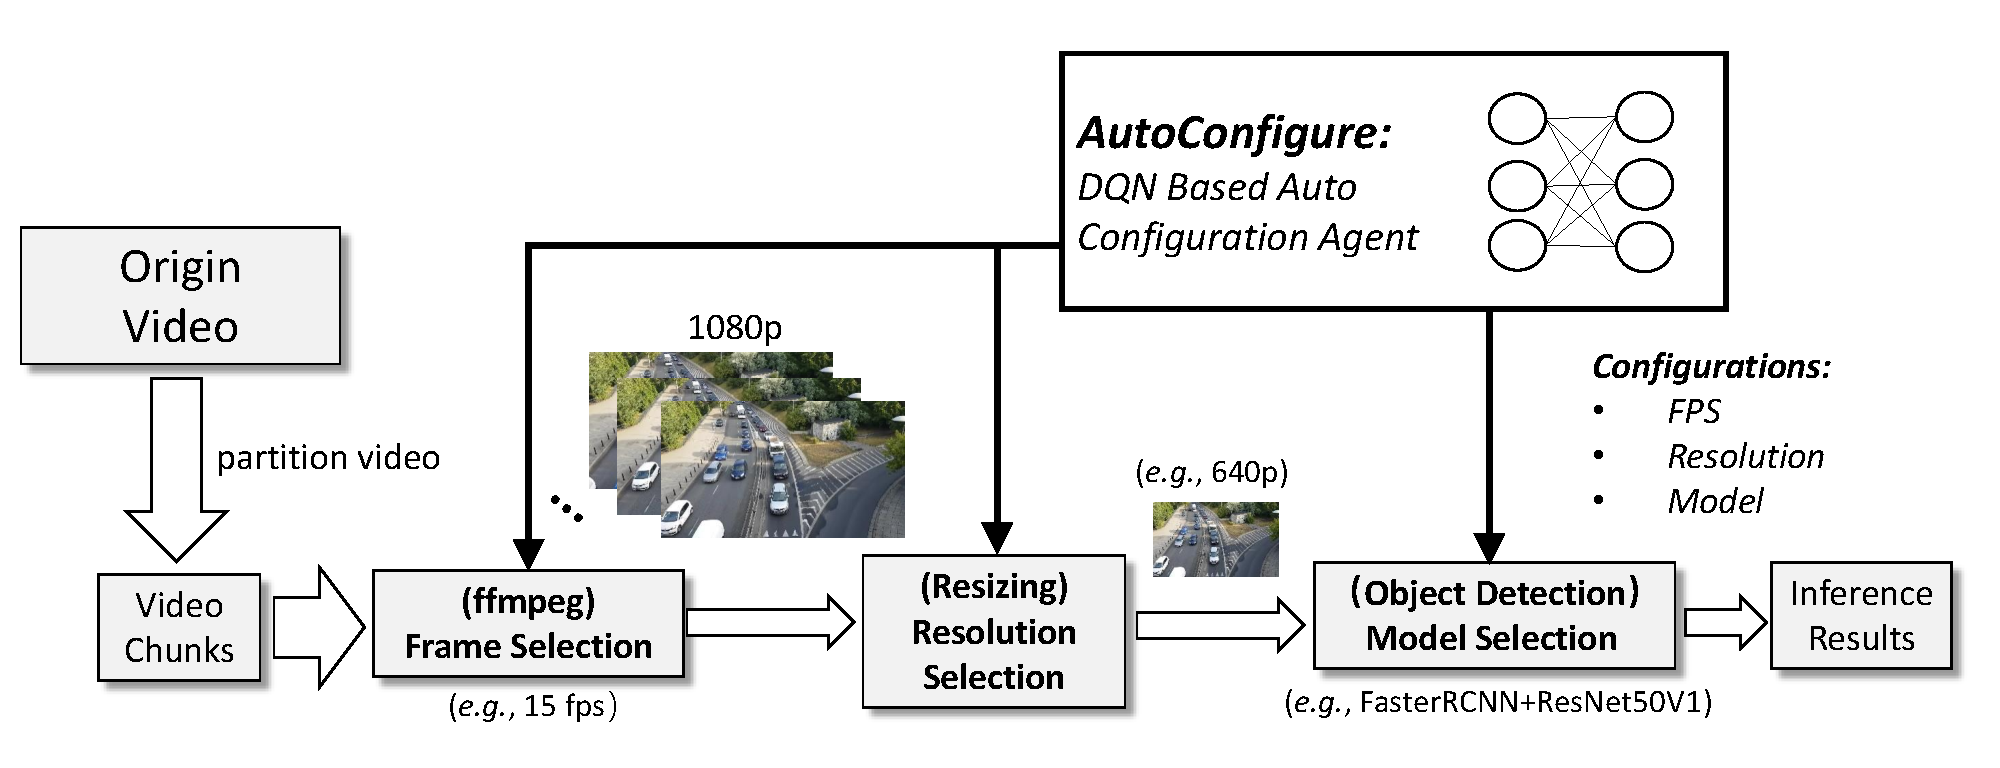
\includegraphics[width=0.9\linewidth]{figures/framework.pdf}}
%	%	\vspace{0.2cm}
%	\caption{Framework of AutoConfigure architecture}
%	\label{fig: framework}
%\end{figure*}

%We use~\autoref{fig2} to support that, the data in this figure come from a real road. It can be found that with the decrease of frame rate, the resource consumption can be significantly reduced, but the reduction of accuracy is partly acceptable.

%As shown in~\autoref{fig1}, at a fixed frame rate, using a complex model with high resolution (such as FasterRCNN+InceptionResnet 1024p) can obviously and accurately detect the target object, but it also requires more computing resources. However, when using the same model, choosing a lower resolution can reduce the computing resources, and the subsequent cost is the decline of accuracy. Another example is that choosing a simple model with low resolution (such as FasterRCNN+ResNet50 640p) can significantly reduce resource consumption, although it reduces the accuracy to some extent.

%\begin{figure}[h]
%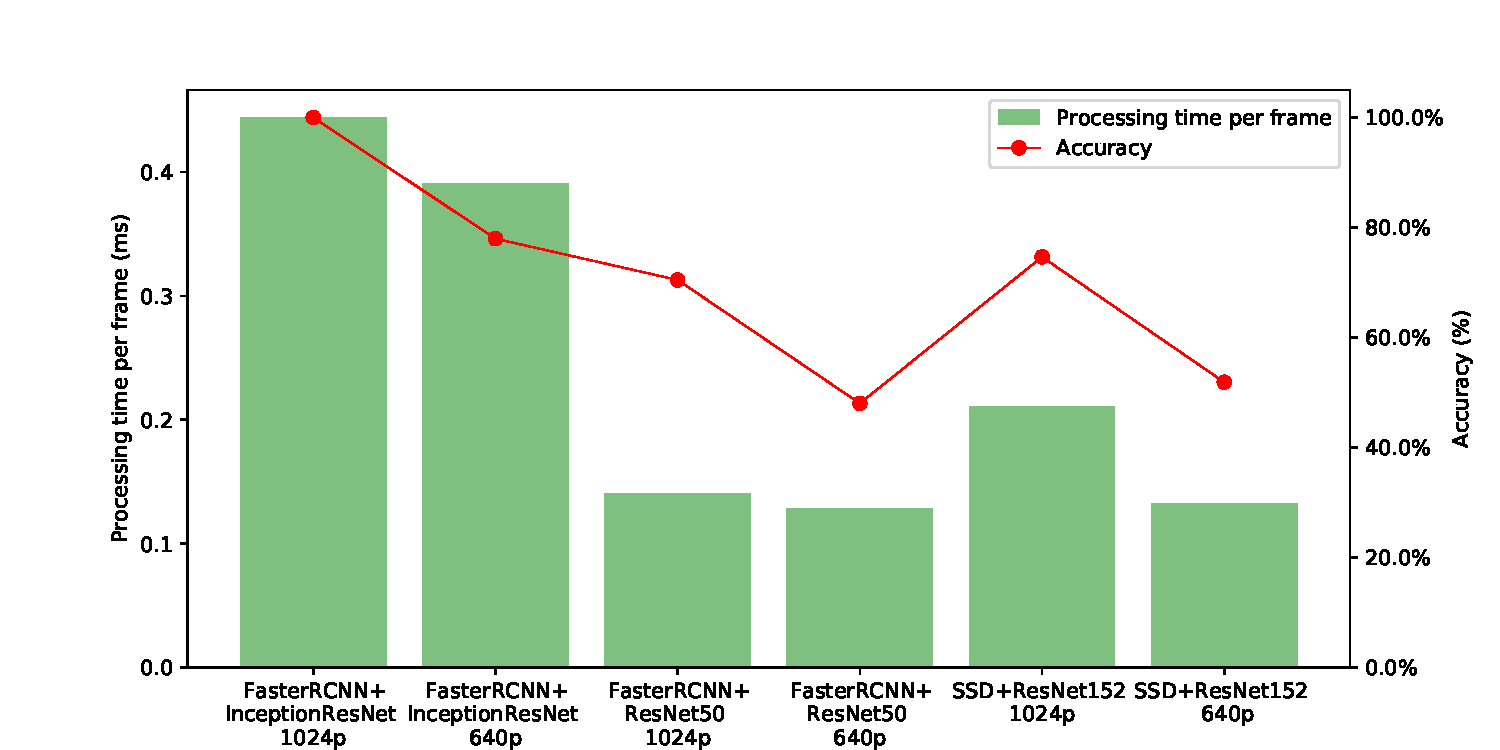
\includegraphics[width=9cm,height=5cm]{figures/figure1.pdf}
%\centering
%\caption{The effect of different models and resolutions on accuracy and processing time at a fixed frame rate.}
%\label{fig1}
%\end{figure}
%
%\begin{figure}[h]
%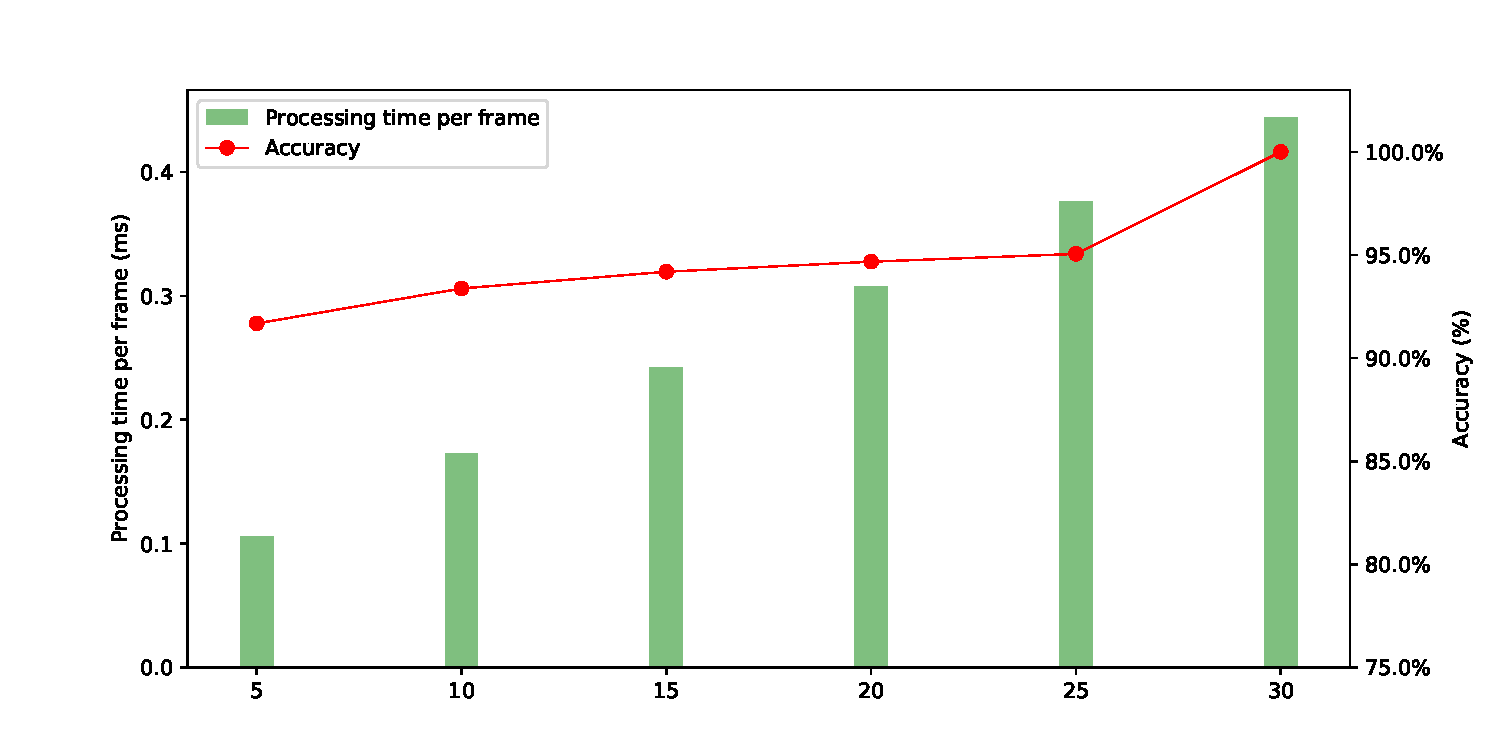
\includegraphics[width=9cm,height=5cm]{figures/figure2.pdf}
%\centering
%\caption{Under the best model, the accuracy and processing time vary with the different frame rate.}
%\label{fig2}
%\end{figure}


%Like figure~\ref{fig: framework}(a), if one just use a unified static configuration solution (i.e.only profiles the processing pipeline to choose the best configuration \emph{once}), the application would either waste resources (by picking an expensive configuration) or sacrifice accuracy (by selecting a cheap configuration).

%Hence, we aim to find a range of ``most appropriate'' configurations that %takes up the
%minimize the consumption of computing resources and is accurate to the desired threshold. On the one hand, like figure~\ref{fig: framework}(a), if one just use a unified static configuration solution (i.e.only profiles the processing pipeline to choose the best configuration \emph{once}), the application would either waste resources (by picking an expensive configuration) or sacrifice accuracy (by selecting a cheap configuration). On the other hand, if one periodically profiles the processing pipeline to find an optimal resource-accuracy \emph{tradeoff} by exhaustive all configurations, it would be prohibitively expensive since the configuration space is extremely large, and thousands of configurations can be combined with just a few knobs. To tackle these challenges, we propose an adaptive configuration approach, AutoConfigure, and the brief framework is shown in Figure~\ref{fig: framework}(b).

%The most intuitive way to solve this problem is to find the best solution by exhaustive all configurations. Still, the number of possible configurations grows exponentially, and thousands of configurations can be combined with just a few knobs, so exhaustive configuration is a highly unrealistic approach.

%For a video analytics application, choosing the ``most appropriate'' configuration is a complicated decision-making problem that is challenging to solve by rules. An adaptive approach is needed to learn from video contexts to decide the best configuration for the current video context. The reinforcement learning method is an excellent way to solve this unsupervised complex-environmental problem. In our solution, we tackle the following design challenges.


%Also, one is not provided the well-labeled data on which configuration should be used at which time of the video, meaning this is an unsupervised learning task.

